\chapter{\hspace*{3pt} Experiments, Results, and Discussion}


\label{chapter:experiments}

This chapter presents the methods, results, and discussion of the experiments that were carried out to verify the validity of the proposed approach. Initially, we describe a proof of concept made by running the classification based on the top-level categories of Wikipedia in posts from ten online Q\&A communities.  We also run an experiment with real users on a crowdsourcing platform to verify if the classification generated by the proposed approach is corroborated by humans, the actual users of information retrieval and organization tools.
Finally, we have used the document representation proposed by our approach in the classification of documents of a classic dataset employing a probabilistic classification algorithm, with the intent to compare and discuss the results regarding a related work.

\section{\hspace*{3pt} Proof of Concept - Q\&A Communities}
\label{section:proof-of-concept}

The first evaluation of our approach is a proof of concept aiming to analyze the classification based on our method in posts of  Q\&A (Question and Answers) communities. 

Q\&A (Question and Answers) have emerged in the past few years as Web 2.0 becomes popular. They provide a place for users to ask specific questions and receive direct answers. 
The users exchange and share their knowledge explicitly by asking or answering questions in a set of predefined topics and categories. 

The volume of questions answered on Q\&A sites so far exceeds the number of questions answered by library reference services \cite{Shah:2010}. As a result, question and answer archives are various knowledge repositories, making it a challenge to organize and retrieve relevant documents in these repositories \cite{Andrzejewski:2009}.


In this context, Stack Exchange\footnote{\url{https://stackexchange.com/}}
is a network of 133 Q\&A communities on topics in varied fields, each community covering a specific theme, where questions, answers, and users are subject to a reputation award process.

For our evaluation, we decided to use Stack Exchange because it covers a wide variety of topics and also because they make data available publicly in a structured way. 

\subsection{\hspace*{3pt} Materials and Methods}

We relied on an anonymized dump of all user-contributed content on the Stack Exchange network, extracted on August 31st 2017\footnote{\url{https://archive.org/details/stackexchange}}. Each site is formatted as a separate archive consisting of XML files from Posts, Users, Votes, Comments, PostHistory and PostLinks. We used the Posts files as the basis for this experiment. As per the description of the dataset, the property postTypeId denotes if the given row in the file is a question or an answer. 

We selected ten representative communities on stack exchange to perform this evaluation: 

Astronomy\footnote{\url{http://astronomy.stackexchange.com}}, 
Biology\footnote{\url{http://biology.stackexchange.com}},
Chemistry\footnote{\url{http://chemistry.stackexchange.com}}, Christianity\footnote{\url{http://christianity.stackexchange.com}}, History\footnote{\url{http://history.stackexchange.com}}, Law\footnote{\url{http://law.stackexchange.com}},Math\footnote{\url{http://mathoverflow.net}}, Music\footnote{\url{http://music.stackexchange.com}}, Philosophy\footnote{\url{https://philosophy.stackexchange.com}} and Sports\footnote{\url{https://sports.stackexchange.com/}}

For each row in the Post.xml file of each one of these communities, we executed the three steps of the chain described in Section \ref{sec:approach}. We first extracted the entities present in each post, than we linked the entities with their categories in DBPedia and finally we traversed the \gls{wcg} by the shortest paths to the top-level categories. 

\subsection{\hspace*{3pt} Results and Discussion}

Table \ref{tab:stackdist} displays the number of posts by type found in the datasets. Note that the column unknown is relative to post that were identified neither as a question nor as an answer. 


\begin{table}[htpb]
\centering
\caption{Distribution of post type in the stack exchange datasets}
\label{tab:stackdist}
\begin{tabular}{@{}llll@{}}
\toprule
Community                            & Questions & Answers & Unknown \\ \midrule
mathoverflow.net.count               & 84657     & 124683  & 1029    \\
chemistry.stackexchange.com    & 23074     & 26997   & 646     \\
biology.stackexchange.com      & 15934     & 19009   & 1068    \\
music.stackexchange.com        & 11101     & 29980   & 770     \\
christianity.stackexchange.com & 9267      & 22043   & 1446    \\
philosophy.stackexchange.com   & 8619      & 20474   & 299     \\
history.stackexchange.com      & 7339      & 14657   & 681     \\
law.stackexchange.com          & 6337      & 7815    & 472     \\
astronomy.stackexchange.com    & 5019      & 7383    & 437     \\
sports.stackexchange.com       & 3711      & 5830    & 656     \\ \bottomrule
\end{tabular}%

\end{table}


In figure \ref{fig:complete-path-count-distribution} we show our results as the aggregated number of shortest paths based on our method from all documents of each dataset to each one of the 19 top-level categories of Wikipedia.
We consider that the distribution of the number of shortest paths among the 19 categories corresponds to the fuzzy distribution of the classification in a given dataset. Thus, the category with the highest number of paths is the one that most contributes to the complete classification.



 \begin{figure}[H]
    \centering
    \begin{subfigure}{0.5\textwidth}
    \centering
        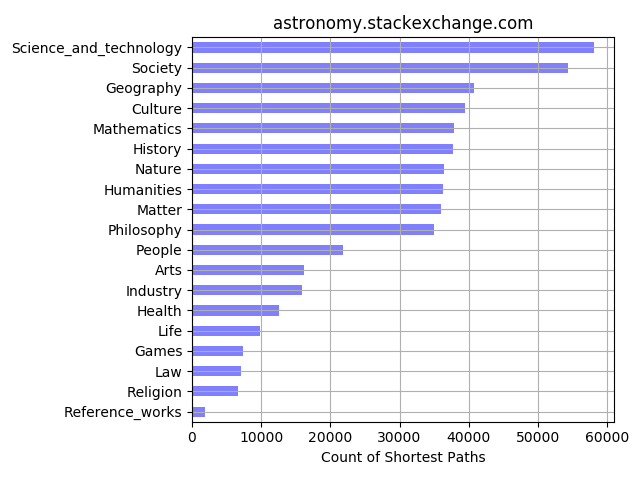
\includegraphics[width=1\linewidth]{imgs/path-counts/astronomy_stackexchange_com}
        \caption{Paths count for Astronomy}
        \label{fig:path-count-astronomy}
    \end{subfigure}%
    \begin{subfigure}{0.5\textwidth}
    \centering
        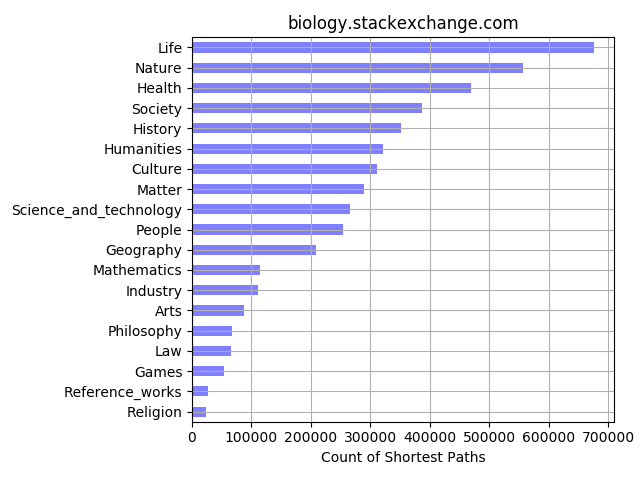
\includegraphics[width=1\linewidth]{imgs/path-counts/biology_stackexchange_com}
        \caption{Paths count for Biology}
        \label{fig:path-count-biology}
    \end{subfigure}
 
     \begin{subfigure}{0.5\textwidth}
    \centering
        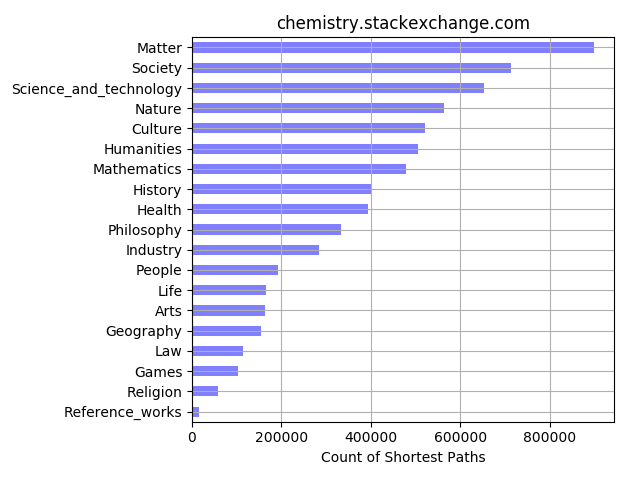
\includegraphics[width=1\linewidth]{imgs/path-counts/chemistry_stackexchange_com}
        \caption{Paths count for Chemistry}
        \label{fig:path-count-chemistry}
    \end{subfigure}%
    \begin{subfigure}{0.5\textwidth}
    \centering
        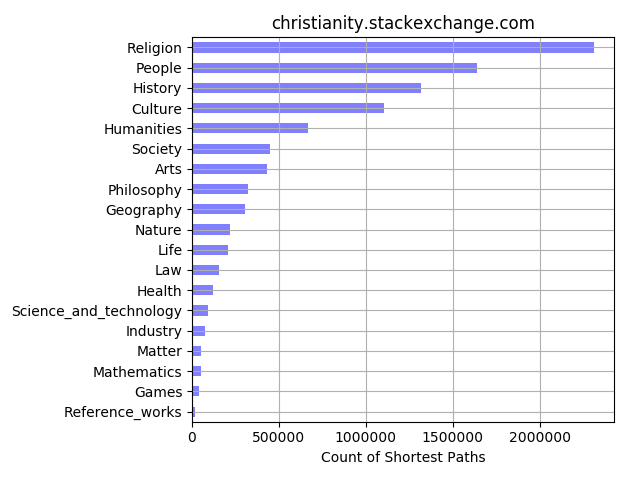
\includegraphics[width=1\linewidth]{imgs/path-counts/christianity_stackexchange_com}
        \caption{Paths count for Christianity}
        \label{fig:path-count-christianity}
    \end{subfigure}

        
     \begin{subfigure}{0.5\textwidth}
    \centering
        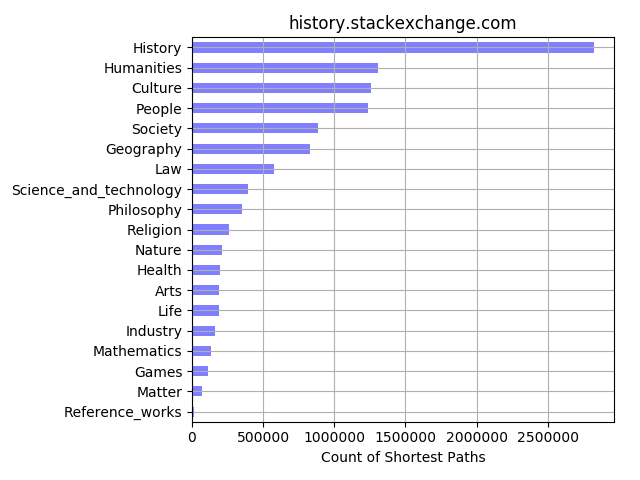
\includegraphics[width=1\linewidth]{imgs/path-counts/history_stackexchange_com}
        \caption{Paths count for History}
        \label{fig:path-count-history}
    \end{subfigure}%
    \begin{subfigure}{0.5\textwidth}
    \centering
        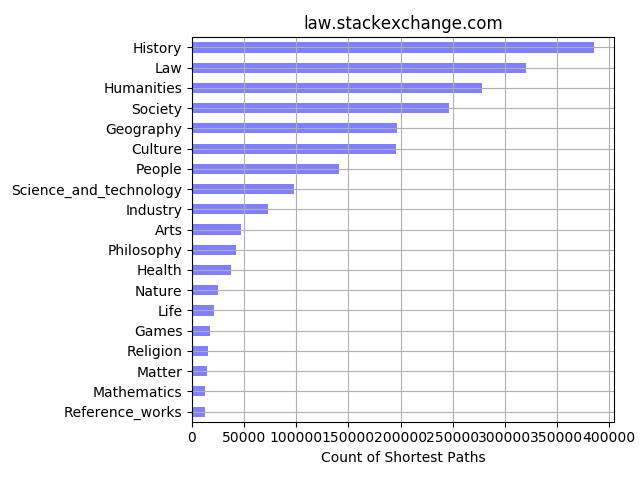
\includegraphics[width=1\linewidth]{imgs/path-counts/law_stackexchange_com}
        \caption{Paths count for Law}
        \label{fig:path-count-law}
    \end{subfigure} 

    \end{figure}
    
 \begin{figure}[H]
 \ContinuedFloat
    \centering
    \begin{subfigure}{0.5\textwidth}
    \centering
        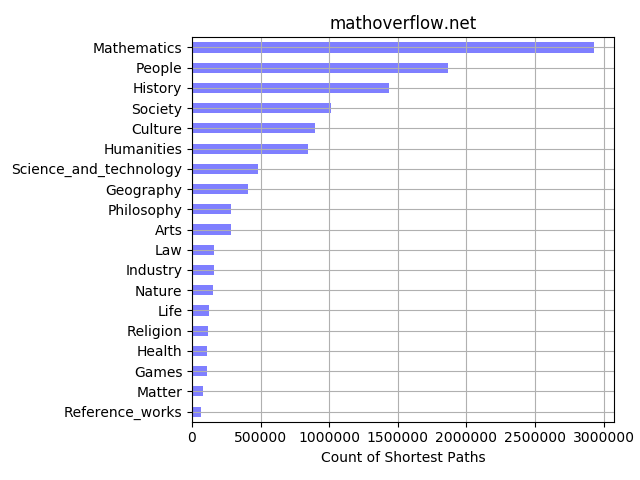
\includegraphics[width=1\linewidth]{imgs/path-counts/mathoverflow_net}
        \caption{Paths count for Math}
        \label{fig:path-count-math}
    \end{subfigure}%
    \begin{subfigure}{0.5\textwidth}
    \centering
        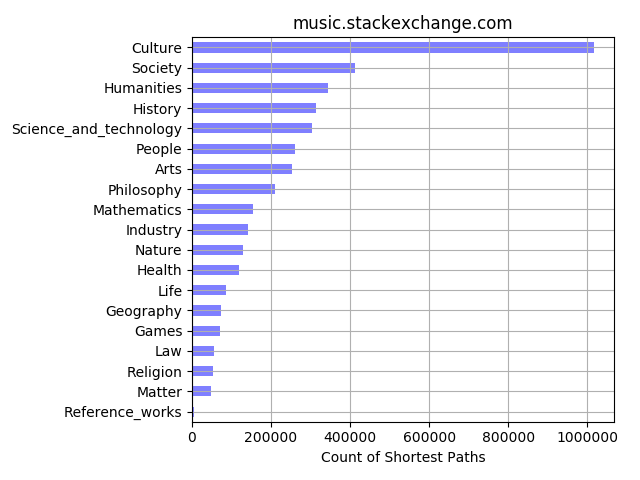
\includegraphics[width=1\linewidth]{imgs/path-counts/music_stackexchange_com}
        \caption{Paths count for Music}
        \label{fig:path-count-music}
    \end{subfigure}
 
     \begin{subfigure}{0.5\textwidth}
    \centering
        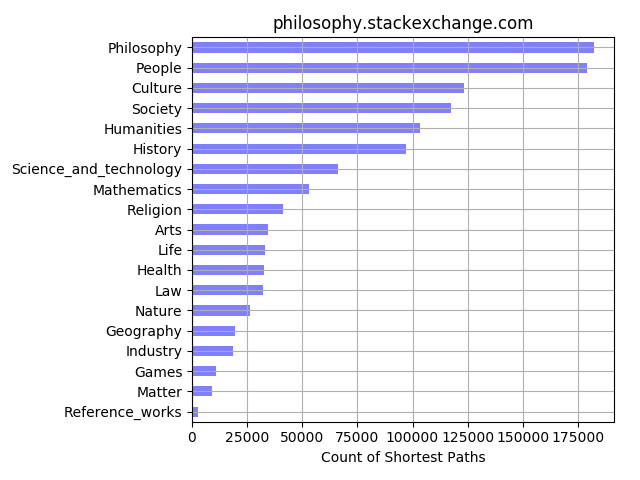
\includegraphics[width=1\linewidth]{imgs/path-counts/philosophy_stackexchange_com}
        \caption{Paths count for Philosophy}
        \label{fig:path-count-philosophy}
    \end{subfigure}%
    \begin{subfigure}{0.5\textwidth}
    \centering
        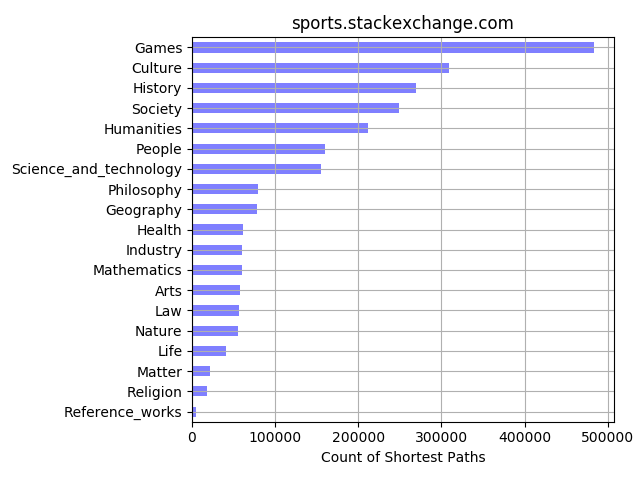
\includegraphics[width=1\linewidth]{imgs/path-counts/sports_stackexchange_com}
        \caption{Paths count for Sports}
        \label{fig:path-count-sports}
    \end{subfigure}
   
 
    \caption{The number of shortest paths through the proposed method. The X-axis shows the number of paths found for each top-level category (displayed on the Y-axis) }
    \label{fig:complete-path-count-distribution}
    
\end{figure}

In the datasets History (\ref{fig:path-count-history}), Mathematics (\ref{fig:path-count-math}) and Philosophy(\ref{fig:path-count-philosophy}) it is possible to see a high level of precision in the classification, considering that the predominant category (the one with more shortest paths) correspond directly to the topic of the community. 

Although the name of the communities does not directly reflect a top-level category of Wikipedia, it can also be considered an accurate result for the datasets Astronomy (\ref{fig:path-count-astronomy}), Biology(\ref{fig:path-count-biology}), Chemistry(\ref{fig:path-count-chemistry}), Christianity(\ref{fig:path-count-christianity}), and Sports(\ref{fig:path-count-sports}).

As per description, the mentioned communities were created so that users can discuss the topics described by the categories whose paths are the most prominent.

For the dataset Music (\ref{fig:path-count-music}) the category with the highest number of shortest paths is Culture. It can be explained first because music is an essential aspect of human society as it is a form of communication and expression.

Moreover, the Culture category comprises in its subcategories several topics that represent aspects related to music, both concerning Music as a form of art (e.g., Music by Genre, Music by Culture, Music in Culture), as well as in the technical aspect of Music as a form of science (e.g., Musical composition, Music Terminology).

Another particular case is the result for the dataset Law (\ref{fig:path-count-law}). As one of the 19 top-level is entitled Law, it was expected that the classification with the highest number of paths would be the category Law. However, the category History appears with a higher degree, while the category Law appears in the second place.

This fact can be explained because both concepts are closely related. The law raises when different events happen over the course of time; These events later come to be known as history. So one can say in both ways either law are a byproduct of history and also the current laws will control the future events which later becomes history.

The example bellow is a real post(answer) extracted from the Law dataset. In this example, it is possible to see how the topic related to Law is also connected to History. While there are the entities \textit{Treaties}, \textit{Court} and \textit{Domestic Law} strongly related to concept of Law, There are also \textit{Sovereign}, \textit{Maastricht Treaty} and \textit{Yugoslavia} that are also related to History. 

\begin{displayquote}
\say{One of the powers that sovereign nations have is to make treaties with other sovereign nations, these can be bi-lateral (as in the example you cite) or multi-lateral (like the Maastricht Treaty that binds the EU together). Once a treaty is agreed and signed it needs to ratified by each country which makes it part of the domestic law in that country: for your example, if India breaches the treaty it can be taken to court under the laws and in the courts of India or Pakistan(...). The worlds newest nation is, I believe, South Sudan, and one that has recently vanished is Yugoslavia. Laws are not contracts: contracts require consent of the parties, among other things., laws don't, they are imposed irrespective of consent.}
\end{displayquote}

\section{\hspace*{3pt} Crowdsourcing study}

In order to verify if the classification generated by the proposed method is coherent for real users, we conducted an experiment with human judges in order to verify how much they agree with the automatic classification result. For this purpose, we use the stack exchange datasets to make the comparison possible with the experiment described in section \ref{section:proof-of-concept}.



\subsection{\hspace*{3pt} Experimental Design}

Due to the accessibility of established micro-task crowd-sourcing platforms such as Amazon’s Mechanical Turk\footnote{\url{www.mturk.com}} and CrowdFlower, researchers are actively turning toward paid crowd-sourcing to solve data-centric tasks that require human input, such as building ground truths, validating results, and curating data \cite{7156008}.

We used CrowdFlower\footnote{\url{http://crowdflower.com}}, an on-line platform which provides access to a workforce to perform tasks.  It automatically allocates the available tasks to contributors and tests them against known answers, named Gold Standard. Their performance on test questions indicates how much the system trusts each contributor and if they become untrusted, they are removed from the task, and the work is discarded.

For this experiment, we also considered as top-level categories the ones defined as Main topic classifications on Wikipedia (19 categories by the date of data extraction). 

For each one of the ten communities, we run the experiment with 200 different random items extracted from the stack exchange dataset. 

We asked each contributor to read texts randomly chosen from the dataset and answer to what extent the text belongs to each one of the categories on a scale ranging from 0 (not at all) to 3 (to a great extent). 

To alleviate the intensive task of judging for 19 Categories, we asked the participants the evaluate the top-3 categories with greatest percentage distribution and two other random categories.  Figure \ref{fig:example-question} shows a real example of task delivered to contributors for the dataset Biology. The categories LIFE, HEALTH and NATURE are the top-3 categories with the highest degree of membership according to our method (see figures \ref{fig:path-count-biology} and \ref{fig:percentage-distribution-biology}). The categories RELIGION and GAMES were randomly introduced in the survey. 

Random categories were included to validate whether, in addition to agreeing with the categories that appear with the highest distribution in the classification, they also agree with those that do not belong to the most prominent categories.  

Moreover, this mechanism reinforces the verification of the validity of the judgments, since random categories cannot have a distribution of responses similar to those in the top-3 categories.

To select the participants able to perform the task proposed in the experiment, we created a series of 30 test questions for the stack exchange dataset, so that the participates with low performance in the test questions were eliminated in this stage.


As described in \cite{Gadiraju:2017}, many research works have referred to the importance of task clarity tangentially and stressed the positive impact of task design, clear instructions and descriptions on the quality of crowdsourced work. 

In this regard, we provided a detailed guide for contributors to make sure they clearly understand how to perform the task, with examples of good and bad judgments and also with a description of each one of the 19 categories. To make sure the task is perfectly designed, CrowdFlower platform offers a consulting service where the top-rated contributors evaluate and give feedback on the quality of a given task. An example of the feedback given by this consulting service can be seen in figure \ref{fig:example-feedback}. 

We adjusted the task description according to the suggestions in the feedback by providing more and contextualized examples, as well as explaining, for each test question, the reason why the alternatives were considered wrong or correct.  

After executing the study with users in the crowdsourcing platform, we performed an analysis in order to verify how much these users agree with the classification generated by our approach in the ten datasets extracted from Q\&A communities.

For this evaluation, we calculated the precision, recall, and F-measure commonly used to verify the quality of information retrieval techniques, including text classifiers\cite{makhoul1999performance}.

Precision measures the number of times a category was correctly predicted by our method (True Positive) divided by the number of times that category was predicted in total (True Positive + False Positive).

To maximize precision, it is necessary that the classifier not misclassify the text entries in the dataset. Texts that should be assigned to one particular category according to the user study must be classified with the same category by our approach.

The main disadvantage of this metric is that it does not take into account the texts that should have been classified in a particular category, but was assigned to another one.

The recall covers this gap by measuring the number of times a category has been assigned to text by users (True Positive + False Negative), but the automatic classifier has not considered classified it correctly (False Negative).

The disadvantage of this metric is that if the automated classifier did not classify any text incorrectly, the recall would be maximum, although it was not efficient (because it also did not sort correctly).

In addition to precision and recall, we have the measure F, which corresponds to the harmonic mean between precision and recall. With this information, we can say the performance of the classifier with an indicator only.

The F-measure metric measures the efficiency of the classifier taking into account the error in both classes (True Positive and False Negative). It is necessary that the adjustment in both classes increase so that the metric increases. 

Considering that F-measure is an average, it gives a more accurate view of the efficiency of the classifier than just precision or recall.

\subsection{\hspace*{3pt} Quality Control}

When dealing with a random collection of strangers to perform relevance evaluation, two primary concerns have risen:  i) How to ensure that contributors performing the evaluation will have the necessary skill or knowledge? ii) How to make sure that the contributors will make a high-quality effort to do the work, rather than clicking randomly on the responses?


To address these questions, we defined some parameters of quality regarding the contributors and the experiment:

\begin{enumerate}

\item We restricted the participation to contributors from English-speaking countries to ensure that they understood the task and instructions adequately. 

\item We restricted the participation to Level-3 contributors on CrowdFlower, meaning that only those who completed over 100 test questions across hundreds of different types of tasks and have a near perfect overall accuracy. They are contributors of the highest quality on CrowdFlower.

\item We restricted each contributor to a maximum of five judgments across all datasets, to minimize the number of contributors trying to complete a massive number of tasks in order to make more money.

\item We predefined the minimum of 0.75 regarding the level of agreement among the contributors for each row of text evaluated. In case a row does not reach this value with the default number of 3 judgments, new judgments were requested until the agreement coefficient reached 0.75.

Before we run the experiment with all ten communities, we first evaluated whether there is a difference between the quality of judgments performed by elite contributors and the judgments made by regular contributors. The elite contributors (also called level-3 contributors in the context of CrowdFlower platform) are those who completed over 100 test questions across hundreds of different types of tasks and have a near perfect overall accuracy. To perform this verification, we ran the experiment using the Biology dataset in two different groups: one only with regular contributors and the other with level-3 contributors. They were asked to judge the same set of 200 questions. 

\end{enumerate}

\subsection{\hspace*{3pt} Results and Discussion}

In the final experiment, 1,265 unique contributors participated from June to August of 2018. The overall setup for the experiment is presented in table \ref{tab:experiment-overview}. A trusted judgment is an answer from a contributor with an accuracy score higher than the minimum accuracy considered for this experiment (0.75), while an untrusted judgment is an answer from a contributor whose accuracy score has fallen below this value.

\begin{table}[H]

\centering
\caption{Overall setup for the experiment with crowd workers}
\label{tab:experiment-overview}
\resizebox{\textwidth}{!}{%
\begin{tabular}{@{}llllll@{}}
\toprule
Community         & Trusted Judgments & Untrusted Judgments & Average Judgments per Row & Average Trust of Workers & Unique Workers \\ \midrule
Astronomy         & 640               & 36                  & 3.2000                    & 0.8651                   & 128            \\
Biology (Elite)   & 612               & 48                  & 3.0600                    & 0.8390                   & 122            \\
Biology (Regular) & 1040              & 278                 & 5.2000                    & 0.8366                   & 208            \\
Chemistry         & 751               & 12                  & 3.7550                    & 0.8197                   & 150            \\
Christianity      & 628               & 16                  & 3.1558                    & 0.8843                   & 125            \\
History           & 602               & 76                  & 3.0251                    & 0.7997                   & 120            \\
Law               & 601               & 0                   & 3.0050                    & 0.8831                   & 120            \\
Math              & 630               & 32                  & 3.1500                    & 0.9306                   & 126            \\
Music             & 602               & 28                  & 3.0100                    & 0.9137                   & 120            \\
Philosophy        & 717               & 108                 & 3.5850                    & 0.8376                   & 143            \\
Sports            & 629               & 32                  & 3.1608                    & 0.8349                   & 125            \\ \bottomrule
\end{tabular}%
}
\end{table}

\subsubsection{\hspace*{3pt} Elite Contributors X Regular Contributors}


A statistical test was applied aiming at determining if the results obtained in the answers given by the two groups can be considered significantly different from each other. The Wilcoxon-Mann-Whitney nonparametric statistical inference test was applied\cite{feltovich2003nonparametric}. This test compares the mean of two independent samples and does not require normality and homoscedasticity in the series of values compared. The level of significance was set at 95\%. The p-value evaluates the result of this statistical test. The lower is the p-value, the higher the significance of the outcome. For a significance level of 95\%, if the p-value is smaller than 0.05, we can conclude that responses observed for the two groups are distinct. 

We obtained a p-value of  0.267 ($\gg 0.05$), meaning that there is no evidence of significant difference between the answers given by the two groups. 

If we analyze the table \ref{tab:experiment-overview} it is possible to see that regular users are less efficient and thus more judgments are needed to achieve a reasonable level of agreement. 

Even though the price paid to regular contributors is lower in comparison to elite contributors, we decided to admit only level-3 users.

\subsubsection{\hspace*{3pt} Human Judgment Analysis}

The figure \ref{fig:complete-crowd-distribution} shows the aggregated results of the participants' judgment regarding the categories in the Q\&A community datasets. The vertical axis presents the five categories involved in each study, three of which correspond to the categories with the highest degree of membership obtained in the experiment described in section \ref{section:proof-of-concept} and the other two were inserted randomly.



 \begin{figure}[H]
    \centering
    \begin{subfigure}{0.5\textwidth}
    \centering
        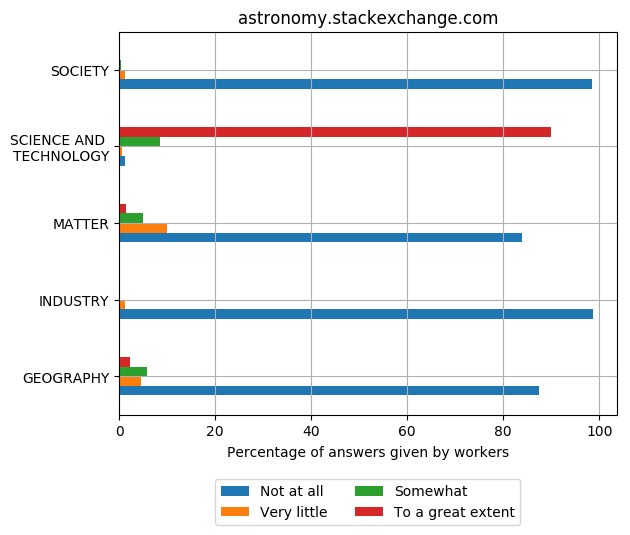
\includegraphics[width=1\linewidth]{imgs/crowd-results/astronomy_stackexchange_com}
        \caption{Distribution of Answers for Astronomy}
        \label{fig:crowd-results-astronomy}
    \end{subfigure}%
    \begin{subfigure}{0.5\textwidth}
    \centering
        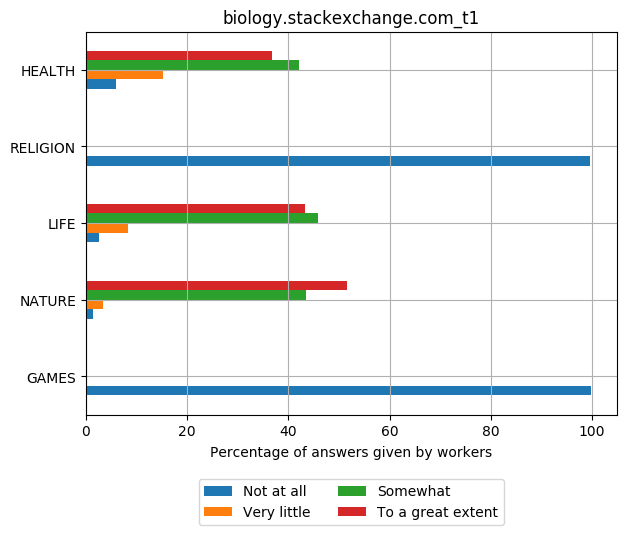
\includegraphics[width=1\linewidth]{imgs/crowd-results/biology_stackexchange_com_t1}
        \caption{Distribution of Answers for Biology (Regular)}
        \label{fig:crowd-results-biology-1}
    \end{subfigure}
 
     \begin{subfigure}{0.5\textwidth}
    \centering
        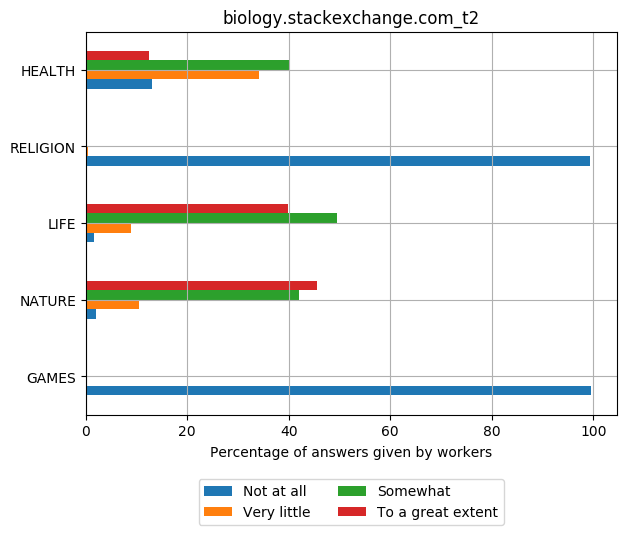
\includegraphics[width=1\linewidth]{imgs/crowd-results/biology_stackexchange_com_t2}
        \caption{Distribution of Answers for Biology (Elite)}
        \label{fig:crowd-results-biology-2}
    \end{subfigure}%
    \begin{subfigure}{0.5\textwidth}
    \centering
        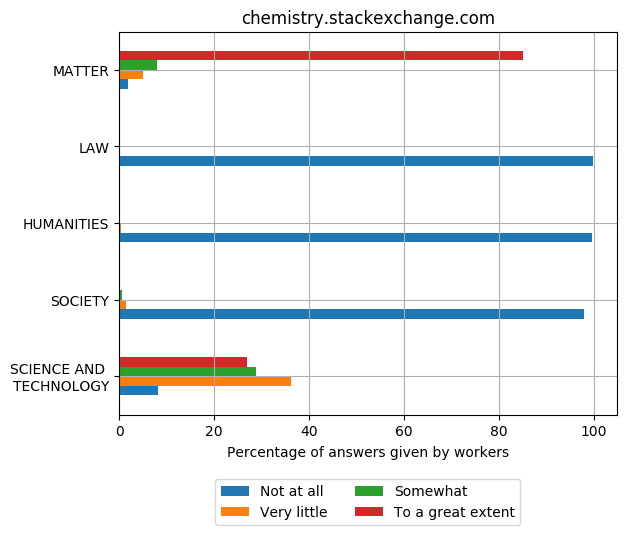
\includegraphics[width=1\linewidth]{imgs/crowd-results/chemistry_stackexchange_com}
        \caption{Distribution of Answers for Chemistry}
        \label{fig:crowd-results-chemistry}
    \end{subfigure}

        
     \begin{subfigure}{0.5\textwidth}
    \centering
        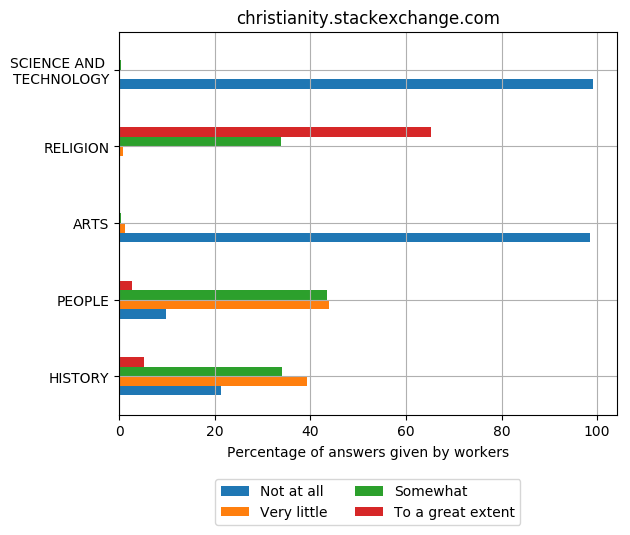
\includegraphics[width=1\linewidth]{imgs/crowd-results/christianity_stackexchange_com}
        \caption{Distribution of Answers for Christianity}
        \label{fig:crowd-results-christianity}
    \end{subfigure}%
    \begin{subfigure}{0.5\textwidth}
    \centering
        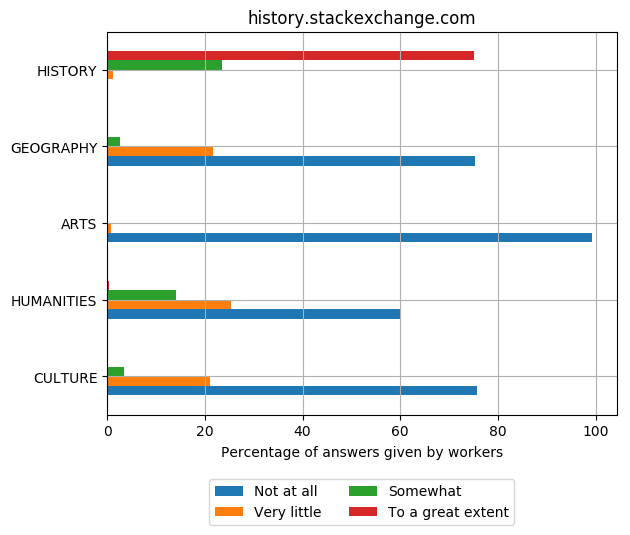
\includegraphics[width=1\linewidth]{imgs/crowd-results/history_stackexchange_com}
        \caption {Distribution of Answers for  History}
        \label{fig:crowd-results-history}
    \end{subfigure} 

    \end{figure}
    
 \begin{figure}[H]
 \ContinuedFloat
    \centering
    \begin{subfigure}{0.5\textwidth}
    \centering
        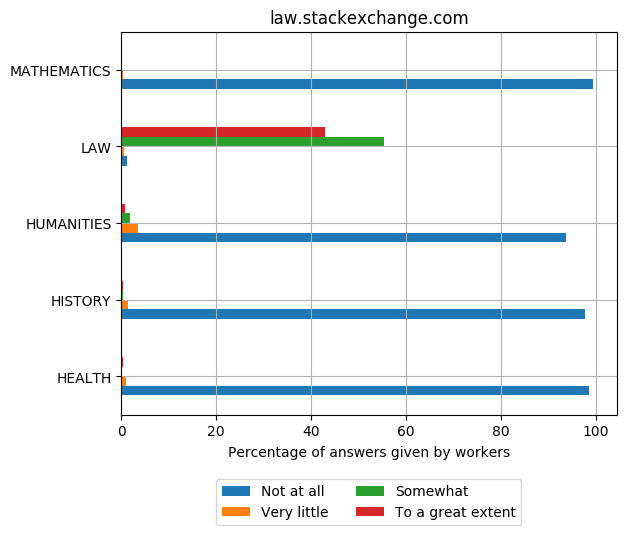
\includegraphics[width=1\linewidth]{imgs/crowd-results/law_stackexchange_com}
        \caption{Distribution of Answers for Law}
        \label{fig:crowd-results-law}
    \end{subfigure}%
    \begin{subfigure}{0.5\textwidth}
    \centering
        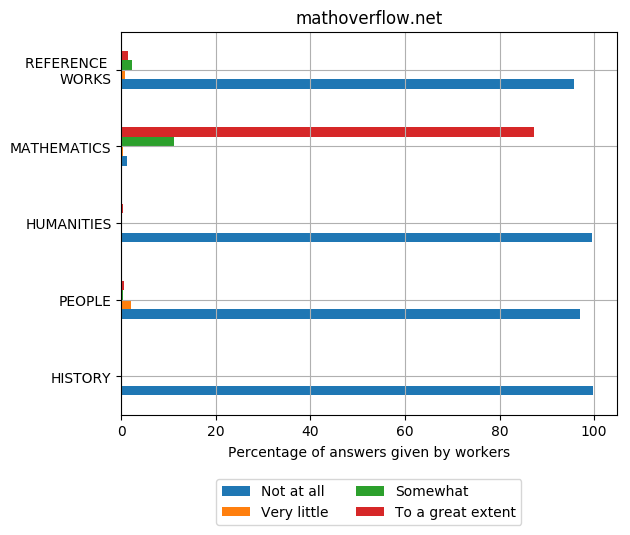
\includegraphics[width=1\linewidth]{imgs/crowd-results/mathoverflow_net}
        \caption{Distribution of Answers for Math}
        \label{fig:crowd-results-math}
    \end{subfigure}
 
     \begin{subfigure}{0.5\textwidth}
    \centering
        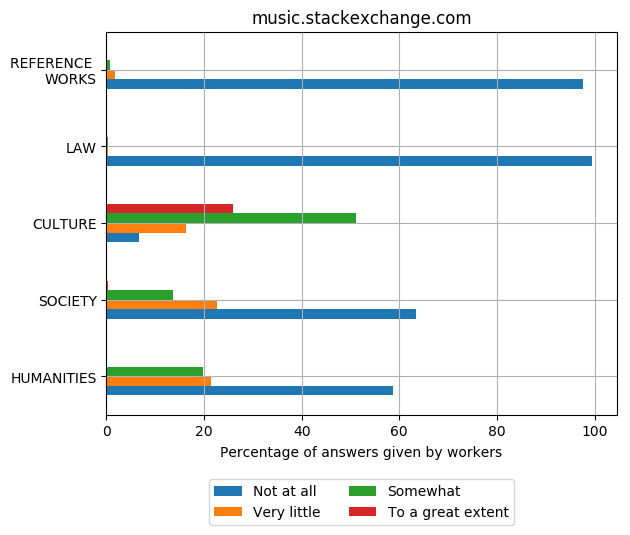
\includegraphics[width=1\linewidth]{imgs/crowd-results/music_stackexchange_com}
        \caption{Distribution of Answers for Music}
        \label{fig:crowd-results-music}
    \end{subfigure}%
    \begin{subfigure}{0.5\textwidth}
    \centering
        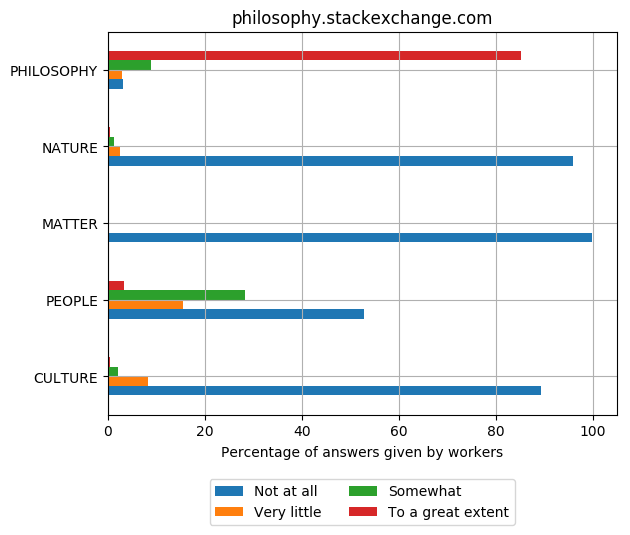
\includegraphics[width=1\linewidth]{imgs/crowd-results/philosophy_stackexchange_com}
        \caption{Distribution of Answers for Philosophy}
        \label{fig:crowd-results-philosophy}
    \end{subfigure}
    
     \begin{subfigure}{0.5\textwidth}
    \centering
        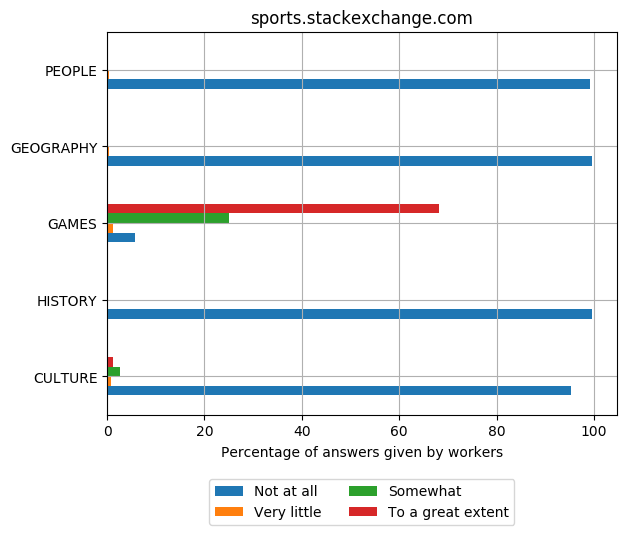
\includegraphics[width=1\linewidth]{imgs/crowd-results/sports_stackexchange_com}
        \caption{Distribution of Answers for Sports}
        \label{fig:crowd-results-sports}
    \end{subfigure}%
 \caption{Percentage distribution of answers given by crowd contributors for each one of the ten communities evaluated }
    \label{fig:complete-crowd-distribution}
    
\end{figure}
 
In the Astronomy(\ref{fig:crowd-results-astronomy}) community, the three most relevant categories were Science and Technology, Society and Geography, respectively. The categories inserted randomly were Industry and Matter.

For the most relevant category (Science and Technology), the vast majority of users agreed with the classification generated by our method (89.86\% To a great extent, 8.52\% somewhat, and 4.57\% Very little).

Although the category Society was the second most relevant according to the automatic classification, it was not identified by the users (87.51\% Not at all). It can be explained by the fact that users identify categories superficially, based on their prior knowledge, but fail to recognize more tacit subjects that permeate the discussions. A good example that justifies the presence of the Society category in the automatic classification is the presence of several inquiries regarding the Geocentric Model, that is linked to the categories History of astrology, History of astronomy and Obsolete scientific theories, indirectly connected to the category Society.
However, users tend to answer that there is no relationship at all to the category Society in these discussions.

Another interesting observation is that although the category Matter is not one of the top 3 most relevant according to our classification, it was identified by some users (9.88\% Very little, 4.94\% Somewhat and 1.35\% To a great extent). One of the reasons that explain this behavior is that there are many discussion in the Astronomy community regarding the existence of carbon, water and other elements in the surface and the atmosphere of planets. 




\begin{table}[H]
\centering
\caption{My caption}
\label{my-label}
\resizebox{\textwidth}{!}{%
\begin{tabular}{@{}lllllll@{}}
\toprule
& \multicolumn{3}{c}{Strict Comparison} & \multicolumn{3}{c}{Flexible Comparison} \\ \midrule
Community                          & Precision    & Recall   & F-Measure   & Precision    & Recall    & F-Measure    \\
astronomy.stackexchange.com        & 0.9423       & 0.2022   & 0.3330      & 0.9872       & 0.1935    & 0.3235       \\
biology.stackexchange.com          & 0.4170       & 0.3311   & 0.3691      & 0.9064       & 0.3492    & 0.5041       \\
chemistry.stackexchange.com.csv    & 0.8571       & 0.3111   & 0.4565      & 0.9524       & 0.3160    & 0.4746       \\
christianity.stackexchange.com.csv & 0.6815       & 0.5951   & 0.6353      & 0.9960       & 0.5731    & 0.7275       \\
history.stackexchange.com.csv      & 0.7528       & 0.6526   & 0.6991      & 0.9925       & 0.6559    & 0.7899       \\
law.stackexchange.com.csv          & 0.0149       & 0.6667   & 0.0292      & 0.0299       & 0.6667    & 0.0571       \\
mathoverflow.net.csv               & 0.8896       & 0.6361   & 0.7418      & 0.9955       & 0.6314    & 0.7727       \\
music.stackexchange.com.csv        & 0.2760       & 0.8019   & 0.4106      & 0.8019       & 0.7816    & 0.7917       \\
philosophy.stackexchange.com.csv   & 0.9081       & 0.3889   & 0.5446      & 0.9622       & 0.3732    & 0.5378       \\
sports.stackexchange.com.csv       & 0.7372       & 0.5479   & 0.6286      & 0.9805       & 0.5331    & 0.6907       \\ \bottomrule
\end{tabular}%
}
\end{table}


\section{\hspace*{3pt} Datasets}

\subsection{\hspace*{3pt} 20 NewsGroups}

The 20 Newsgroups dataset is a collection with approximately 20,000 documents from the UseNet discussion forum. The documents in this collection are divided into 20 categories related to the following subjects: computers, business, religion, politics, science, and fun. The distribution of documents among categories is regular, i.e., categories have approximately the same number of documents, and each document belongs to only one category.


\begin{figure}[H]
\centering
  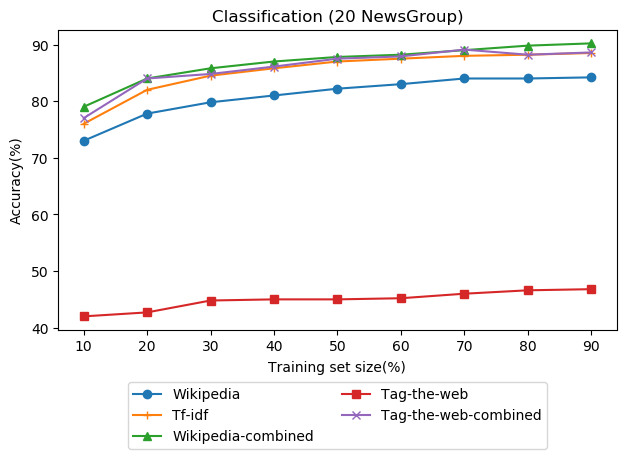
\includegraphics[width=\linewidth]{comparison.png}
  \caption{Classification accuracy in 20 Newsgroups at various training set sizes compared to \cite{schonhofen2009identifying} }
  \label{fig:example-comparison}
\end{figure}
